\vspace{-6ex}
\section{Buchmarkt}
\vspace{-3ex}
\begin{multicols*}{2}
\begin{wrapfigure}[12]{r}{0cm}
	\fibelimgtext[above right]{
		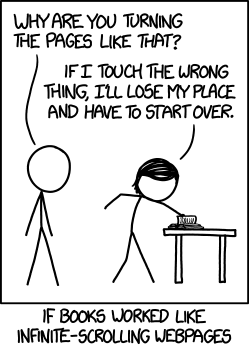
\includegraphics[width=4cm]{res/xkcd/1309_infinite_scrolling.png}
	}{\url{https://xkcd.com/1309}}
\end{wrapfigure}
% XXX Jedes Jahr das Buchmarkt-Datum aktualisieren!
Am 25.10.2016 veranstalten wir (die Fachschaft) wieder für euch (die Studenten) einen Buchmarkt.
Der Buchmarkt bietet euch die Möglichkeit, günstig an gute Fachbücher zu kommen.
Die Bücher stammen von älteren Studenten oder aus dem alten Bestand der Studierendenbibliothek der Fachschaft.
Die meisten Bücher sind zwar nicht mehr ganz neu, aber dafür recht günstig und in gutem Zustand.

Wir bieten euch Bücher zu verschiedenen Themen, wie z.\,B.\ Mechanik, Elektrodynamik, Chemie oder auch Mathematik.
Aber auch zu anderen Bereichen gibt es interessante Bücher.
Leider gibt es meist nur ein Exemplar.
Daher gilt das Motto: Wer zuerst kommt, mahlt zuerst.

Von dem eingenommenen Geld der Fachschaftsbücher werden wieder neue Bücher angeschafft, welche ihr im Lernzentrum (AP-Bib) zur Verfügung gestellt bekommt.
Somit profitiert ihr doppelt von dem Kauf der Bücher.
Wer auf der Suche nach interessanten Büchern ist, oder auch nach Büchern, die einem beim Studium nützlich sein können, ist beim Buchmarkt genau richtig.

Der Buchmarkt findet immer Anfang des Wintersemesters statt -- achtet einfach auf unsere Plakate, E-Mails und Ankündigungen in den Vorlesungen!

\fibelsig{Alex}
\end{multicols*}

